\chapter{Methodology}\label{chapter:Methodology}
This chapter proposes an algorithm, which overcomes the restrictions of the ortho algorithm reviewed as state of the art in chapter \ref{chapter:SotA}. Therefore three different signal distribution networks are introduced. Namely an ordering, a majority gate and a sequential distribution network. The name signal distribution networks refers to the fact, that the algorithm still works in the same fashion as the original ortho algorithm, only redistributing signals, when implementing irregularities, therefore changing the layout in a way the irregular parts fit with the regular placement and routing. The irregularities are based on the ordering of inputs, placement of majority gates and sequential circuitry parts. Because only 2DD-Wave clocking is used for the ortho algorithm, the signal distribution networks can also change the clocking in order to implement the new functionalities they provide. In the following first the ordering distribution network is discussed, which aims to reduce area in the input region of the layout. Afterwards the networks used for implementing majority gates and sequential parts are discussed and analyzed.

\section{Ordering Distribution Network}
Looking again at the resulting layout of a 2:1 mux or ortho in \ref{fig:ortho_mux_21}, it can be seen that in the first few rows, where the primary inputs are placed, no other gates are put, because the space has to be reserved for rewiring in order to solve conflicts. The idea of the ordering distribution network is to allow gates also to be placed in this area to save space and placing inputs in a way that wire crossings may be minimized. To do so the ordering network has to resolve the conflicts in some other way. Recalling the pseudo-code from the ortho algorithm, an input has a conflict when it is colored south because it is not allowed to wire over the other inputs laying in the same column. This means the area overhead in the input region is highly dependent on the coloring assigned to the outgoing edges of the inputs. The algorithm used in the pseudo-code line $3$ is implemented in a way that just finds \textit{some} valid but not an \textit{optimal} coloring for the given logic network. Unfortunately due to the algorithms nature it often assigns the color south to exactly these edges resulting in the said area overhead. Therefore the first step is to improve the coloring of the logic network and prevent excess wiring. Secondly a new rule for edges colored south inside the conflicting area can be introduced, making the rewiring redundant. The third idea, which can be implemented in the network is an ordering of the inputs in order to allow those who are connected with the same gates to be placed near each other reducing wire expenses and crossings.

\begin{algorithm}[H]
	\vdots
	
	\begin{algorithmic}
		\State Convert $N$ to a 3-graph by substitution and balance inverters at fan-out nodes
		\State Order primary input nodes
		\State \vdots
		\State Generate \textbf{conditional} direction assignment $d : \Delta \rightarrow \{east, south\}$ and subdivide signals if necessary
		\State Compute topological ordering $v_1, . . . , v_i \in N$
		\State Extend $L$ by one column and reserve it for primary inputs
		\ForAll {vertex $v_1, ..., v_i \in N $ with at most two incoming signals $\sigma_1, \sigma_2$}
		\If{vertex $v$ is terminal/primary input}
		\State Extend $L$ by one row
		\State Place v at position $(0, h - 1)$
		\ElsIf{$d(\sigma_1) = d(\sigma_2) = east$}
		\State \vdots
		\ElsIf { signals are labeled $south$}
		\If{\textbf{not} root node exists}
		\State Extend $L$ by one row
		\EndIf
		\State $w_p \leftarrow$ max. horizontal position of v's predecessors
		\State Place v at position $(w _p, h - 1)$
		\EndIf
		
		\EndFor
		\State \vdots \\
		\Return $L$
	\end{algorithmic}
	\caption{Ortho changes with ordering distribution network}\label{alg:input_network}
\end{algorithm}

To discuss the idea, first the parts of the logic network, which belong to the ordering distribution network have to be determined. This can be deduced from looking at the layout, where the wasted area appears for mostly the primary inputs and nodes connected to them. Thus, all primary inputs and the gates which they are wired to, skipping over inverters, are viewed as part of the ordering distribution network. Skipping means that if the outgoing edge of an primary input is an inverter, the gate hanging on the outgoing edge of the inverter is considered. Starting with the different gates inputs can be connected to, the coloring they can have should be discussed. The direction assignment of one-input nodes including inverters and fan-out nodes can be chosen arbitrarily because the primary input they are connected to has always only one outgoing edge, resulting in no dependencies. In this case always the non-conflicting $east$ assignment can be chosen. When looking at two-input logic gates like AND and OR gates it has to be seen that the coloring can only be chosen arbitrarily if both input nodes are primary inputs, allowing again the non-conflicting assignment of $east$. In every other case the direction assignment has to consider the coloring of the other incoming edge of the gate. In order find out the dependencies, the ordering distribution network places first every primary input connected to a fan-out node with its respective fan-out node itself into the layout. This has several advantages. First of all the fan-out nodes give the constraints for the conditional coloring, which is introduced in the ordering distribution network. Also fan-out nodes produce new paths and therefore excess wiring, which means that their dependencies should be resolved as fast as possible by placing and routing them to their outgoing gates as fast as possible. Following the coloring rules, two outgoing edges of a node need to be colored with different directions, so that the fan-out gates placed into the network have one output assigned with color $east$ and one output assigned with color $south$. Considering that the second coloring constraint requires the other incoming edge of the gate connected to the $south$ colored edge, also to be colored $south$ and the second incoming edge being connected to a primary input, we can see that a conditional coloring alone is not powerful enough to resolve all conflicts. For this case a new placement rule for the $south$ coloring is introduced in order to preserve the direction assignment rules but still resolve the conflict between primary inputs. The original algorithm part (line 14-22) handling the placement of nodes based on their coloring makes sure that every gate placed $east$ occupies a new column and every node colored $south$ occupies a new row. These placement rules allow every gate to be placed without interfering with other gates, but the rules have been found to be to restrictive, allowing the following placement rule for $south$. If a node is labeled south and its predecessor, which has the lower horizontal position \textbf{also} has the higher vertical position, it is called the \textit{root node} and the layout is \textbf{not} extended by a column while the gate is still placed to position $(w_p, h-1)$. Following this rule the gate is now placed in the same column as its predecessor with the higher y-coordinate. If we apply this to a two-input gate in the ordering distribution network with a primary input and a fan-out node as predecessors, the primary input is always the root node due to the ordering and new coloring. Thus, the new rule allows the two-input gate connected to the $south$ colored primary input and the fan-out node to be placed in the same column as the primary input, resulting in no conflict because the node is not \textit{actually} placed southern of its predecessors. It was found that this rule could not only be utilized for this special case but also for the general $south$ placement in the algorithm with one exception. Considering a fan-out node to be the root node, the coloring would wire both the eastern and the southern colored outgoing edges onto the same row, yielding a conflict. The resulting pseudo-code snippets replacing the used code are shown in algorithm \ref{alg:input_network}. Also it has to be considered that the conditional coloring in the distribution network still needs to include helping nodes e.g. when three fan-out nodes are connected to each other. Also before the coloring, first the input nodes need to be ordered according to the ideas presented. Thus, primary input nodes connected to fan-out nodes are placed first and then the primary input nodes, which are connected to the outgoing edges of the fan-out nodes are placed. This is done to reduce the distance between coherent gates and therefore also the number of wire crossings. Afterwards primary inputs directly connected to a gate which has its other incoming edge connected to a second primary input are placed. Finally all input nodes, which are not connected to the rest of the ordering distribution network are placed arbitrarily and the logic network is topologically ordered according to the new order of the primary inputs.
\begin{figure}
	\centering
	\includegraphics[scale=0.5]{input_network_mux_21}
	\caption{Placement and routing of a 2:1 mux network using the ortho algorithm with the ordering distribution network}\label{fig:input_network_mux_21}
\end{figure}
Some other issues are related to inverter nodes. As already mentioned they are skipped in the view of the ordering distribution network, but still need to be considered for the placement and routing. Assuming an inverter node which is assigned $south$ e.g. after a fan-out node and it should be placed in the same row as an primary input, a conflict arises because the input always has to wire east first. Thus, all inverters colored $south$ need to be placed to minimum the row of the most southern primary input plus one. In order to prevent to much overhead produced by inverters a balancing network is introduced, which aims to reduce the number of inverters in the logic network. Based on the substitution of the logic network into $N$ with inverter and fan-out nodes in some cases a fan-out node has two inverters connected to its outgoing edges. Then these inverters are substituted by one single inverter as incoming node to the fan-out, resulting in an overall lower number of inverter nodes.
Figure \ref{fig:input_network_mux_21} shows the placement and routing of the ortho algorithm after implementing the proposed ordering distribution network. The ordering of the inputs puts first the fan-out node and then the two connected primary inputs. In this case the ordering distribution network also considered the inverter at the outgoing edge to be colored east in order to produce less overhead, because if the inverter would be colored $south$ it would have to be placed underneath the primary inputs. Looking at the AND gate connecting the fan-out with the second primary input, we can see that the new rule for nodes placed south is used. This also applies for the AND gate connecting the third primary output to the inverter. The last OR gate is placed after the normal rules of the ortho algorithm. In the comparison to the layout in figure \ref{fig:ortho_mux_21} can be quickly seen that the resulting layout saves up place and even wire crossings. The exact results are presented and analyzed in the next chapter.

\section{Majority Gate Distribution Network}
In this section the placement and routing of majority gates, using the ortho algorithm is discussed and a distribution network is proposed. Because the majority function in QCA can be realized with only a single gate, in theory QCA has a huge advantage to CMOS technology. The introduction of this distribution network allows an analysis of how efficient these majority gates can be implemented in the QCA domain and if their theoretical superiority can be taken advantage of.
\subsection{The proposed signal distribution Network}
Since the ortho algorithm only allows 2DDWave clocking, only the placement of 2-input logic gates is supported and the direction assignment contains only two directions $east$ and $south$. In order to introduce majority gates into layouts a RES-like clocking needs to be utilized. This means, that the layout includes tiles which have three incoming tiles and one outgoing tiles. In the RES scheme in figure \ref{subfig:RES} this tile is on position $(1, 1)$. However, just supporting RES clocking in the ortho algorithm would be quite inefficient and could not be easily implemented. If the clocking would be completely changed to RES, the algorithm could not utilize every row and column of the clocking since the RES scheme also supports signals to flow into western or northern direction. In RES only the first and third row such as the second and fourth column support eastern and southern signal propagation, so only these part of the clocking would be utilized for the placement of two input gates. Also for the placement of three input majority gates a new direction assignment would have to be introduced to the logic network, changing the theory which underlies the ortho algorithm. Another idea would be to support RES clocking in permanently assigned regions, supporting majority gates just in certain places. For this the layout could be devised into $4x4$ sub-regions and e.g. every fifth sub-region would be RES clocked and the rest would be occupied with the 2DDWave scheme. On the one hand this realization should not produce that much area overhead since only some regions could not be utilized for two input logic gates, but the permanent clocking assignment only allows the placement of majority gates in exactly these permanent spots, leading again to large area overhead if a majority gate should be placed in a 2DDWave clocked sub-region. Also the ortho algorithm makes use of the trivial global synchronization constraints within a uniformly 2DDWave clocked layout. By introducing irregular clocking e.g. RES sub-regions, signals can pass a different amount of tiles in order to reach the same tile, therefore violating the global synchronization constraint. Figure !! a RES sub-region embedded in a 2DDWave clocked layout. Drawing the paths from three synchronous starting points to the three input tile, it can be seen, that the paths have different lengths, violating the design rules.


\begin{figure}
	\centering
	\includegraphics[scale=0.8]{Maj_nw}
	\caption{Proposed majority gate distribution network}\label{fig:QCA_Maj_nw}
\end{figure}


To avoid these drawbacks, the proposed distribution network should allow a custom clocking only in areas where majority gates are placed and find a solution for the global signal synchronization constraint. Therefore the placement and routing of solely two input gates should not produce any excess area. Figure \ref{fig:QCA_Maj_nw} shows the proposed majority gate signal distribution network, which is implemented into the ortho algorithm. Although no area overhead is produced for the already existing placement and routing, it can already be seen that the distribution network itself produces excess area due to its complex wiring, resulting again from the conditions that had to be considered designing it. The implementation of an AIG representation of the majority function implemented with ortho is depicted next to the distribution network to visualize that the placement and routing of this single majority gate barely safes area, although it has to be highlighted that no wire crossings are used. Again a comparison of these two implementations can only be done under a cost function representing wire crossings in cost of normal gates.
In the following the design constraints used to design the signal distribution network are discussed. Firstly the distribution network should not contain any wire-crossings, since they are considered to be very costly. Introducing a cost-metric for wire-crossings may result in a more efficient implementation, but for this work wire-crossings should be excluded as design rule for the network. Secondly, the distribution network needs to meet the global synchronization constraint. Considering a 2DDWave clocked layout, every diagonal is synchronous and every signal wired on the same diagonal passes the same amount of tiles following the ortho placement and routing. If we look at the incoming tiles of a three input tile, it can be seen that only two of the incoming tiles are on the same diagonal and the third one is basically shifted by half a clock cycle. This means that this signal is delayed by half a clock cycle violating the global synchronization constraint. Also in order to support the further use of 2DDWave and the local synchronization constraint, the signals need to pass a multiple of whole clock cycles in the signal distribution network. Therefore the first the other two incoming signals are delayed by half a clocking signal, meeting the global synchronization constraint at the tile, where the majority gate is places. Afterwards the signal again is delayed by half a clock cycle so it can be connected to the regular 2DDWave clocking scheme. From this explanation it can be derived that every signal representing a majority gate is delayed by one clock cycle compared to the remaining layout. This delay no has to be considered for each gate placed after the placement and routing of a majority gate distribution network. In the following first the basic placement and routing of the majority gate distribution network and then the solution for meeting the global synchronization constraint in further placement and routing is discussed. 

\subsection{Placement and routing}
The placement and routing of the proposed signal distribution network is again bound to some constraints. First of all the coloring of majority gates has to be reviewed, since the logic network now includes three input nodes. However the coloring algorithm can include helping nodes to resolve coloring conflicts of edges and therefore dividing every edge with a helping node allows a trivial coloring also for three input nodes. Another aspect regarding coloring was the need for a new direction in order to connect a third signal to the majority gate. But since the only occasion such a wiring happens is inside the fixed distribution network, which again can be placed and routed in the usual manner, no additional directions need to be included. Another aspect which has to be reviewed is the irregular clocking inside the signal distribution network. These irregularities don't allow the algorithm to wire connections over the network. From the algorithms perspective a majority gate cannot be placed just south or east of another gate because these gates again could need a wiring through the majority gate distribution network. Therefore the algorithm is forced to assign the distribution network always south and east direction to prevent routing conflicts. Even though this comes again with a non-optimal use of area, this supports the trivial coloring assignment discussed above. This also allows the coloring to be included into the input ordering distribution network, so that all inputs connected to a majority gate need to be colored $east$.

\subsection{Signal synchronization and buffer insertion}
The placement and routing results in a delay of one clock cycles of signals passing through a majority gates. Since the tile-based clocking doesn't support a speedup of a signal, every other signal which comes into contact with a delayed signal also has to be delayed. Therefore an algorithm is introduced in order to compute the delay of signals and allowing signals which are connected together to be synchronized by buffer insertion. For the delay computation, the algorithms views every incoming edge from a node starting at the primary output. If an incoming edge is connected to a majority gate every other incoming edge gets a delay assigned. In this way delays are only inserted when signals are connected together in contrast to just delaying every other signal in the network. The delay is realized by inserting a buffer, except all incoming edges are delayed, meaning they are still synchronous. When placing a gate the delay can be therefore maximum one clock cycle. Figure \ref{fig:QCA_buf} depicts a buffer in east direction, which can be used also in southern direction by just rotating it by 90 degrees. The snake-like structure delays a signal by exactly one clock cycle and is also used in the placement and routing resulting from the QCA ONE library \cite{QCA_scl}. As in the majority gate distribution network, the buffers support irregular clocking, which has to be considered within the algorithm, because signals cannot pass through these areas. In the case of buffers only one column or row is made impassable, allowing to track them and introducing a rewiring for conflicts. Figure \ref{fig:majority_with_buf} shows the placement of a majority gate inside the input distribution network and two and gates which have to be delayed in order to be connected with the delayed signal comming out of the majority gate distribution network. The insertion of the first buffer blocks the eastern direction of the second input. For this case a resolve column is introduced where the signal can be assigned to a new row and be wired without conflict. From this layout it can already be seen that the implementation of the majority gate distribution network brings several complications with it, all resulting in area overhead, which stands in contrast to the area which should be saved by introducing majority gates in the first place.

\begin{figure}
	\centering
	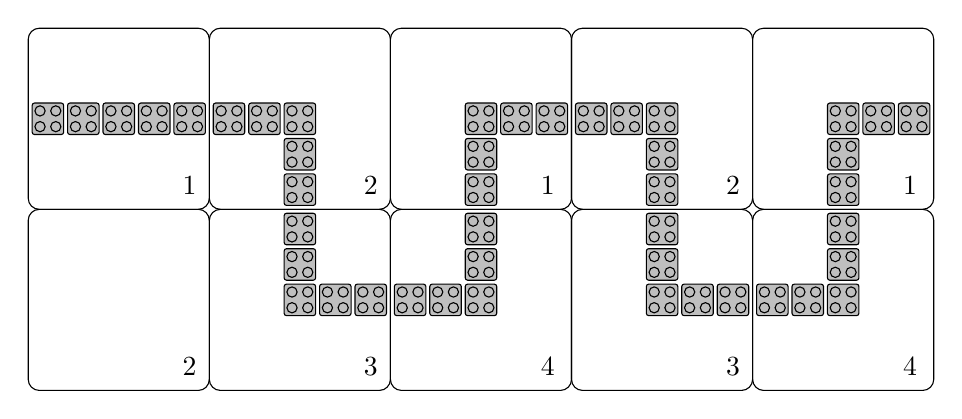
\begin{tikzpicture}
	\begin{scope}[xshift=-2.3cm, rotate=90]
		\draw[rounded corners] (-0.05, -0.1 - 0.85) rectangle (2.3-0.05, 2.3-0.1 - 0.85){};
		
		\foreach \x/\y in {0.9/0.9, 0.9/0.45, 0.9/0, 0.9/-0.45, 0.9/-0.9}
		{
			\draw[rounded corners = 0.3mm, fill=lightgray] (\x, 0 + \y) rectangle (1.2/3 + \x, 1.2/3 + \y){};
			\draw (0.3/3+ \x,0.3/3 + \y) circle (0.65mm);
			\draw (0.9/3+ \x,0.3/3+ \y) circle (0.65mm);
			\draw (0.3/3+ \x,0.9/3 + \y) circle (0.65mm);
			\draw (0.9/3+ \x,0.9/3 + \y) circle (0.65mm);
		}
	\node[text=black] (A1) at (0.25,-0.7) {$1$};
	\end{scope}
	\begin{scope}[xshift=-2.3cm, yshift=-2.3cm, rotate=90]
		\draw[rounded corners] (-0.05, -0.1 - 0.85) rectangle (2.3-0.05, 2.3-0.1 - 0.85){};
		
		\node[text=black] (A1) at (0.25,-0.7) {$2$};
	\end{scope}
	\begin{scope}[shift={(0, 0)}, rotate=90]
			\draw[rounded corners] (-0.05, -0.1 - 0.85) rectangle (2.3-0.05, 2.3-0.1 - 0.85){};
			
			\foreach \x/\y in {0.9/0.9, 0.9/0.45, 0.9/0, 0/0, 0.45/0}
			{
				\draw[rounded corners = 0.3mm, fill=lightgray] (\x, 0 + \y) rectangle (1.2/3 + \x, 1.2/3 + \y){};
				\draw (0.3/3+ \x,0.3/3 + \y) circle (0.65mm);
				\draw (0.9/3+ \x,0.3/3+ \y) circle (0.65mm);
				\draw (0.3/3+ \x,0.9/3 + \y) circle (0.65mm);
				\draw (0.9/3+ \x,0.9/3 + \y) circle (0.65mm);
			}
			\node[text=black] (A1) at (0.25,-0.7) {$2$};
	\end{scope}
	\begin{scope}[xshift=3.2cm, yshift=1.3cm, rotate=180]
		\draw[rounded corners] (-0.05, -0.1 - 0.85) rectangle (2.3-0.05, 2.3-0.1 - 0.85){};
		
		\foreach \x/\y in {0.9/0.9, 0.9/0.45, 0.9/0, 0/0, 0.45/0}
		{
			\draw[rounded corners = 0.3mm, fill=lightgray] (\x, 0 + \y) rectangle (1.2/3 + \x, 1.2/3 + \y){};
			\draw (0.3/3+ \x,0.3/3 + \y) circle (0.65mm);
			\draw (0.9/3+ \x,0.3/3+ \y) circle (0.65mm);
			\draw (0.3/3+ \x,0.9/3 + \y) circle (0.65mm);
			\draw (0.9/3+ \x,0.9/3 + \y) circle (0.65mm);
		}
		\node[text=black] (four) at (0.25 ,1.05) {$1$};
	\end{scope}
	\begin{scope}[xshift=-0.4cm, yshift=-0.1cm, rotate=270]
		\draw[rounded corners] (-0.05, -0.1 - 0.85) rectangle (2.3-0.05, 2.3-0.1 - 0.85){};
		
		\foreach \x/\y in {0.9/0.9, 0.9/0.45, 0.9/0, 0/0, 0.45/0}
		{
			\draw[rounded corners = 0.3mm, fill=lightgray] (\x, 0 + \y) rectangle (1.2/3 + \x, 1.2/3 + \y){};
			\draw (0.3/3+ \x,0.3/3 + \y) circle (0.65mm);
			\draw (0.9/3+ \x,0.3/3+ \y) circle (0.65mm);
			\draw (0.3/3+ \x,0.9/3 + \y) circle (0.65mm);
			\draw (0.9/3+ \x,0.9/3 + \y) circle (0.65mm);
		}
		\node[text=black] (A1) at (1.1+0.85,1.1) {$3$};
	\end{scope}
	\begin{scope}[xshift=1cm, yshift=-1.4cm, rotate=0]
		\draw[rounded corners] (-0.05, -0.1 - 0.85) rectangle (2.3-0.05, 2.3-0.1 - 0.85){};
		
		\foreach \x/\y in {0.9/0.9, 0.9/0.45, 0.9/0, 0/0, 0.45/0}
		{
			\draw[rounded corners = 0.3mm, fill=lightgray] (\x, 0 + \y) rectangle (1.2/3 + \x, 1.2/3 + \y){};
			\draw (0.3/3+ \x,0.3/3 + \y) circle (0.65mm);
			\draw (0.9/3+ \x,0.3/3+ \y) circle (0.65mm);
			\draw (0.3/3+ \x,0.9/3 + \y) circle (0.65mm);
			\draw (0.9/3+ \x,0.9/3 + \y) circle (0.65mm);
		}
		\node[text=black] (four) at (1.95 ,-0.65) {$4$};
	\end{scope}

\begin{scope}[xshift=4.6cm, yshift=0cm, rotate=90]
	\draw[rounded corners] (-0.05, -0.1 - 0.85) rectangle (2.3-0.05, 2.3-0.1 - 0.85){};
	
	\foreach \x/\y in {0.9/0.9, 0.9/0.45, 0.9/0, 0/0, 0.45/0}
	{
		\draw[rounded corners = 0.3mm, fill=lightgray] (\x, 0 + \y) rectangle (1.2/3 + \x, 1.2/3 + \y){};
		\draw (0.3/3+ \x,0.3/3 + \y) circle (0.65mm);
		\draw (0.9/3+ \x,0.3/3+ \y) circle (0.65mm);
		\draw (0.3/3+ \x,0.9/3 + \y) circle (0.65mm);
		\draw (0.9/3+ \x,0.9/3 + \y) circle (0.65mm);
	}
	\node[text=black] (A1) at (0.25,-0.7) {$2$};
\end{scope}
\begin{scope}[xshift=7.8cm, yshift=1.3cm, rotate=180]
	\draw[rounded corners] (-0.05, -0.1 - 0.85) rectangle (2.3-0.05, 2.3-0.1 - 0.85){};
	
	\foreach \x/\y in {0.9/0.9, 0.9/0.45, 0.9/0, 0/0, 0.45/0}
	{
		\draw[rounded corners = 0.3mm, fill=lightgray] (\x, 0 + \y) rectangle (1.2/3 + \x, 1.2/3 + \y){};
		\draw (0.3/3+ \x,0.3/3 + \y) circle (0.65mm);
		\draw (0.9/3+ \x,0.3/3+ \y) circle (0.65mm);
		\draw (0.3/3+ \x,0.9/3 + \y) circle (0.65mm);
		\draw (0.9/3+ \x,0.9/3 + \y) circle (0.65mm);
	}
	\node[text=black] (four) at (0.25 ,1.05) {$1$};
\end{scope}
\begin{scope}[xshift=4.2cm, yshift=-0.1cm, rotate=270]
	\draw[rounded corners] (-0.05, -0.1 - 0.85) rectangle (2.3-0.05, 2.3-0.1 - 0.85){};
	
	\foreach \x/\y in {0.9/0.9, 0.9/0.45, 0.9/0, 0/0, 0.45/0}
	{
		\draw[rounded corners = 0.3mm, fill=lightgray] (\x, 0 + \y) rectangle (1.2/3 + \x, 1.2/3 + \y){};
		\draw (0.3/3+ \x,0.3/3 + \y) circle (0.65mm);
		\draw (0.9/3+ \x,0.3/3+ \y) circle (0.65mm);
		\draw (0.3/3+ \x,0.9/3 + \y) circle (0.65mm);
		\draw (0.9/3+ \x,0.9/3 + \y) circle (0.65mm);
	}
	\node[text=black] (A1) at (1.1+0.85,1.1) {$3$};
\end{scope}
\begin{scope}[xshift=5.6cm, yshift=-1.4cm, rotate=0]
	\draw[rounded corners] (-0.05, -0.1 - 0.85) rectangle (2.3-0.05, 2.3-0.1 - 0.85){};
	
	\foreach \x/\y in {0.9/0.9, 0.9/0.45, 0.9/0, 0/0, 0.45/0}
	{
		\draw[rounded corners = 0.3mm, fill=lightgray] (\x, 0 + \y) rectangle (1.2/3 + \x, 1.2/3 + \y){};
		\draw (0.3/3+ \x,0.3/3 + \y) circle (0.65mm);
		\draw (0.9/3+ \x,0.3/3+ \y) circle (0.65mm);
		\draw (0.3/3+ \x,0.9/3 + \y) circle (0.65mm);
		\draw (0.9/3+ \x,0.9/3 + \y) circle (0.65mm);
	}
	\node[text=black] (four) at (1.95 ,-0.65) {$4$};
\end{scope}
		
	\end{tikzpicture}
	\caption{Buffer in $east$ direction with resolve column and respective clocking}\label{fig:QCA_buf}
\end{figure}

\begin{figure}
	\centering
	\includegraphics[scale=0.5]{majority_with_buf}
	\caption{Placement and routing of a majority distribution network in conjunction with two primary inputs}\label{fig:majority_with_buf}
\end{figure}


\section{Sequential Distribution Network}

Importance of sequential circuits.\\
Point out how the registers are implemented.\\
Show how the distribution network is generated, where Ris and Ros are placed and how they are treated within the network.\\
Make clear that this implementation is slowing down the circuit significantly.